\chapter{Performance analysis}
\label{chapter:analysis}

We will now look at the performance profile of various network
configurations.

As we are running these benchmarks on the Mininet software simulator, there
are natural limits on how realistic the results will be.  However, we should
be able to get good \textit{relative} results.   Therefore we will first
need to establish a baseline to which we will compare the
Paxos\index{Paxos!performance} implementation.

Instructions on how to run these tests are given in
\ref{chapter:appendix.benchmark} \vpageref{chapter:appendix.benchmark}.
\todo{Når ferdig, test med ekte software som MySQL, osv osv.}

\section{Baseline --- ICMP ping on L2 learning switch}
\label{chapter:baseline.benchmark}

All our network configurations use the L2 learning switch\index{switch!L2 learning} from chapter
\ref{chapter:l2.learning.switch} to forward packets on the network.  We can
therefore use a setup consisting of switches and this switch as a bsis for
our performance tests.  We will use the topology in figure
\ref{figure:baseline.topology} and send \ac{ICMP} ping\index{ping} packets from one end of
the network to the other.\footnote{
The reason for removing the fall-back link between $S_1$ and $S_3$ in figure
\ref{figure:graph.three.switches} is to prevent the packets from taking
different paths on the network.}

\begin{figure}[ht]
  \centering
  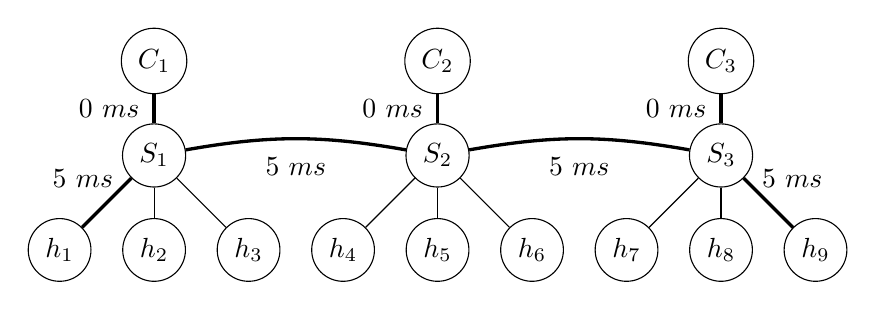
\begin{tikzpicture}[
    every node/.style={draw, circle},
    x=0.6cm,
    y=0.6cm]

    % Switches
    \foreach \n in {1,2,3} {
      \pgfmathsetmacro\x{(\n-2)*6}

      % Switch
      \node (S\n) at (\x ,  0) {$S_\n$};

      % Controller
      \node (C\n) at (\x ,  2) {$C_\n$};
      \draw (S\n) -- (C\n);

      % Hosts
      \foreach \h in {1,2,3} {
        \pgfmathsetmacro\pos{(\h - 2)*2}
        \pgfmathtruncatemacro\num{((\n - 1)*3) + int(\h)}

        % Host node
        \node (h\num) at (\x + \pos, -2) {$h_{\num}$};
        \draw (S\n) -- (h\num);
      }
    }

    % Switch links
    \draw (S1) to[out=10,in=170]
               node[below=-0.2cm, draw=none] {$5~ms$} (S2);

    \draw (S2) to[out=10,in=170]
               node[below=-0.2cm, draw=none] {$5~ms$} (S3);

    % Mark traversal path
    \draw [very thick] (h1) -- node[above left=-0.1cm,draw=none] {$5~ms$} (S1);
    \draw [very thick] (S1) -- node[left,draw=none] {$0~ms$} (C1);
    \draw [very thick] (S1) to[out=10,in=170] (S2);

    \draw [very thick] (S2) -- node[left,draw=none] {$0~ms$} (C2);
    \draw [very thick] (S2) to[out=10,in=170] (S3);

    \draw [very thick] (S3) -- node[left,draw=none] {$0~ms$} (C3);
    \draw [very thick] (S3) -- node[above right=-0.1cm,draw=none] {$5~ms$} (h9);
  \end{tikzpicture}
  \caption{Baseline topology with three switches $S$ and their controllers
           $C$. Node $h_1$ will send ICMP ping packets to $h_9$.
           The packets will go through four links with a configured
           latency of $5~ms$ and back again.
           We assume that link-latencies between switches and
           controllers are practically near zero.}
  \label{figure:baseline.topology}
\end{figure}

The first ICMP ping request from $h_1$ will cause all switches to
rebroadcast the packet to all their ports.  When the ping reaches $h_9$,
it will send back a reply, causing all controllers to learn both
the source and destination ports for $h_1$ and $h_9$.
At this point in time, the controllers can install flow table entries to
automatically forward packets to the known ports.

We will run the test twice: Once using flow tables for forwarding, and once
without.  When not using flows, the controller will issue a \textit{forward
packet to port} to the switch for each packet.

\subsection{Linear relationship of expected \acs{RTT}}

Before we present the results, let's look at what we should expect from the
configuration above \cite{DBLP:conf/cnsm/PhemiusB13}.

Using the link-latency\index{link-latency} $L$ and node
processing\index{processing-delay} time $P$, and a constant $K$ for
background noise, we would expect the \acf{RTT}\index{round-trip time}
between $h_1$ and $h_9$ to be

\begin{gather}
  RTT_{h_1, h_9} = 2\left( \sum_n^4 L_n + \sum_n^3 P_{S_n} + \sum_n^3 P_{C_n} \right) + P_{h_1} + P_{h_9} + K
  \label{equation:baseline.rtt}
\end{gather}

We can simplify by assuming that the controller processing time $P_C$ will
be negligible when complete flow entries have been installed, as the
switches will then handle the forwarding themselves.  During this initial
ramp-up, $L_{C,S} \to 0$ as $P_C \to 0$.  We will also ignore the few
cycles spent on ICMP-processing, setting $P_{h_1}$ and $P_{h_9}$ to zero.
As we will not attempt to measure $K$, we will simply set it to zero as
well.

Using the link latencies $2\sum_n^4 L_n = 2\cdot4\cdot\ms{5} = \ms{40}$
and our simplifications above,
\begin{align}
  RTT_{h_1,h_9} &= \ms{40} + 2\sum_n^3 P_{S_n} + 2\sum_n^3 P_{C_n} \\
                &= \ms{40} + 6P_S + 6P_C
  \label{equation:expected.baseline.rtt}
\end{align}

\subsection{Results}

Results for the two tests are shown in table
\ref{table:rtt.baseline.summary} and figure
\ref{figure:baseline.combined.summary.plot}.

\begin{figure}
  \centering
  \includegraphics[width=\textwidth]{data/pings-combined-summary.pdf}
  \caption{\acs{RTT}s for baseline test.  Medians are shown in red and means
    in blue.
    These plots do not show the large \acs{RTT}s during ramp-up.
    The first row shows \acs{RTT} for switches using flow table entries for
    packet forwarding.  The second row are measurements when using the
    controller to forward packets.  The last row plots both of them.}
  \label{figure:baseline.combined.summary.plot}
\end{figure}

\input{data/pings-combined-summary.tex}

There is a noticeable ramp-up as port numbers are learned and packets are
rebroadcast.  After some time, the \acs{RTT}s seem to get more steady.
Because of this short period of high \acs{RTT}s---compared to the total number of
samples---we will use the \textit{median} as a more realistic value for the
RTT. We also see that the RTT is consistently above the theoretical minimum
of $\ms{40}$.

Using the median RTT\index{round-trip time} for the first run (with flows)
in equation \ref{equation:expected.baseline.rtt}, we can estimate $P_S$.

\input{data/pings-results.tex}

The value for $P_S$ in the first run should be very near the value for the
second run, because the switch still needs to forward packets.  The only
difference between the runs is that, in the first, it must perform a flow
table match, and in the second, it must forward the packet to the
controller.  We will therefore use the value of $P_S$ in the first run to
estimate $P_C$ in the second run.

\input{data/pings-noflows-results.tex}

Again, we would like to reiterate that we are running these tests on a
\textit{simulator}.  That is why the results match so well with the expected
\acs{RTT}.  We also made a \textit{Q-Q plot}\index{Q-Q plot} (see
fig.~\ref{figure:pings.qqplot}) to see if the samples were normally
distributed, and---indeed---they match perfectly (except for the ramp-up
phase).

\begin{figure}
  \centering
  \includegraphics[width=\textwidth]{data/pings-qqplot.pdf}
  \caption{Q-Q plot for ICMP ping RTT (ms).}
  \label{figure:pings.qqplot}
\end{figure}

This is most likely because the underlying simulator uses some
\acf{PRNG}\footnote{Or other, implicit means.} to produce simulated latencies.  But our
benchmarks will still be useful to us.  Using the same topology and link
latencies, we can easily see what kind of implementation techniques that
will make the system more responsive.

\section{L2 learning switch, key-value store}
\label{chapter:benchmark.l2.kv.noflows}

First we need a baseline\index{benchmark!baseline}.  Here we have a topology
of two switches $S_0$ and $S_1$ with a controller each.  The switches has
three hosts, $h_0, \dots, h_5$.  A client $h_1$ is connected to $S_0$. We're
running Python key-value-stores on each host, and $h_1$ will issue a
get-request followed by a put-request to the host $h_5$, which is connected
to $S_1$.  We measure the time for each request, divide it by two and call
it latency.\footnote{We basically assume that the packets take an equal
  amount of time back and forth, and divide by two to get this time.}

There are two controllers $C_0$ and $C_1$ for the switches $S_0$ and $S_1$,
respectively.  In this situation, the packets from $h_1$ need to travel
through two switches.

The network is running on Mininet\index{Mininet}, a software network simulator, on a Linux
virtual machine running on an Mac OS X\index{OS X} box.  All the links in Mininet have
been set up with $10 Mbit/s$ bandwidth\index{bandwidth}, $5~ms$
latency\index{latency}  and no packet
loss.  These links have been set up with \ac{HTB}\index{hierarchical token
bucket} \cite{devera2002hierarchical} enabled, which Open vSwitch\index{Open
vSwitch} uses for providing rate limiting.

In this first benchmark, the switches will send each packet up to the
controllers.  The controllers implement L2 learning switches\index{switch!L2 learning}
and will not install any flow table entries for rapid dispatch.

On the X-axis is the time in seconds.  On the Y-axis is the
latency\index{latency} for get and put requests.

The result can be seen in figure \ref{benchmark:l2.learning.switch.no.flows} 
\vpageref{benchmark:l2.learning.switch.no.flows}.

What is surprising here is that the put-requests have much higher latency
than the get-requests. We don't know why this is.\todo{Finn ut! Er det pga
  pakkene er større? Eller andre grunner?}

\section{L2 learning switch, key-value store, flow entries}

We have the same setup as above, but this time we install flow entries that
will automatically forward the packets.  The flow table entries will match
on as many fields in the packets as possible.

The flow table entries have idle and hard timeouts set to 10 seconds.
In other words, we should be able to see some increased latency every ten
seconds.

% Present both plots together
\begin{figure}
  \centering
  \begin{subfigure}{\textwidth}
    \centering
    \includegraphics[width=\textwidth]{data/data2.eps}
    \caption{L2 learning switch without using flow tables.}
    \label{benchmark:l2.learning.switch.no.flows}
  \end{subfigure}

  \centering
  \begin{subfigure}{\textwidth}
    \centering
    \includegraphics[width=\textwidth]{data/data3.eps}
    \caption{L2 learning switch using flow tables.}
    \label{benchmark:l2.learning.switch.with.flows}
  \end{subfigure}
\end{figure}

The result can be seen in figure \ref{benchmark:l2.learning.switch.with.flows}
\vpageref{benchmark:l2.learning.switch.with.flows}.

Here we can see that the latency has been reduced somewhat.\todo{Hvor mye?
Hva med å plotte over hverandre, hva med å lage average eller root mean
square eller noe sånn?}

We also see some latency spikes around every ten seconds, as expected.

\todo{Plott med flere verdier, istedenfor å vise seconds på x-aksen kan vi
  vise elapsed time, som i at den starter på 0 sekunder.}

These two benchmarks will serve as a baseline to which we will compare our
performance when we enable Paxos on the switches.

Remember that when we run Paxos, we will still have to use the L2 learning
switch for the nodes to be able to communicate.

\todo{Trendlinjner, moving average, fitting osv... må ha det i grafene, må
  også ha litt statistisk analyse av tallene selv osv.}

\section{Three switches, Paxos on controller}

\todo{Få data}

\section{Three switches, Paxos on controller and flow table}

\todo{Få data}

\section{Other solutions}

We chose to use OpenFlow as the basis for our system.
We could just as well have used a networking system that already supported
programmability in some way, for instance the Intel DPDK\todo{Needs
citation}.\todo{Also needs defense.}

\todo{Flytt evt dette ned til improvements-delen}
